\documentclass[16pt]{article}
\usepackage{lmodern}
\usepackage{amssymb,amsmath}
\usepackage{ifxetex,ifluatex}
\usepackage{fixltx2e} % provides \textsubscript
\ifnum 0\ifxetex 1\fi\ifluatex 1\fi=0 % if pdftex
  \usepackage[T1]{fontenc}
  \usepackage[utf8]{inputenc}
\else % if luatex or xelatex
  \ifxetex
    \usepackage{mathspec}
  \else
    \usepackage{fontspec}
  \fi
  \defaultfontfeatures{Ligatures=TeX,Scale=MatchLowercase}
\fi
% use upquote if available, for straight quotes in verbatim environments
\IfFileExists{upquote.sty}{\usepackage{upquote}}{}
% use microtype if available
\IfFileExists{microtype.sty}{%
\usepackage[]{microtype}
\UseMicrotypeSet[protrusion]{basicmath} % disable protrusion for tt fonts
}{}
\PassOptionsToPackage{hyphens}{url} % url is loaded by hyperref
\usepackage[unicode=true]{hyperref}
\hypersetup{
            pdftitle={Root Locus: Example 1},
            pdfborder={0 0 0},
            breaklinks=true}
\urlstyle{same}  % don't use monospace font for urls
\usepackage{graphicx,grffile}
\makeatletter
\def\maxwidth{\ifdim\Gin@nat@width>\linewidth\linewidth\else\Gin@nat@width\fi}
\def\maxheight{\ifdim\Gin@nat@height>\textheight\textheight\else\Gin@nat@height\fi}
\makeatother
% Scale images if necessary, so that they will not overflow the page
% margins by default, and it is still possible to overwrite the defaults
% using explicit options in \includegraphics[width, height, ...]{}
\setkeys{Gin}{width=\maxwidth,height=\maxheight,keepaspectratio}
\IfFileExists{parskip.sty}{%
\usepackage{parskip}
}{% else
\setlength{\parindent}{0pt}
\setlength{\parskip}{6pt plus 2pt minus 1pt}
}
\setlength{\emergencystretch}{3em}  % prevent overfull lines
\providecommand{\tightlist}{%
  \setlength{\itemsep}{0pt}\setlength{\parskip}{0pt}}
\setcounter{secnumdepth}{0}
% Redefines (sub)paragraphs to behave more like sections
\ifx\paragraph\undefined\else
\let\oldparagraph\paragraph
\renewcommand{\paragraph}[1]{\oldparagraph{#1}\mbox{}}
\fi
\ifx\subparagraph\undefined\else
\let\oldsubparagraph\subparagraph
\renewcommand{\subparagraph}[1]{\oldsubparagraph{#1}\mbox{}}
\fi

% set default figure placement to htbp
\makeatletter
\def\fps@figure{htbp}
\makeatother


\title{Root Locus: Example 1}
\date{}

\begin{document}
\maketitle

%\href{http://lpsa.swarthmore.edu/Root_Locus/RLocusExamples.html}{\includegraphics{./Root Locus_ Example 1_files/UniBack.png}}

\section{Root Locus: Example 1}\label{root-locus-example-1}

\subsection{Transfer function}\label{transfer-function}
$\displaystyle G(s)H(s)= \frac{1}{s(s+3)}$
%\includegraphics{./Root Locus_ Example 1_files/imgAC.png}

\subsection[Xfer Function
Info]{\texorpdfstring{\protect\hypertarget{BckGrnd}{}{}Xfer Function
Info}{Xfer Function Info}}\label{xfer-function-info}

For the open loop transfer function, G(s)H(s):\\
We have n=2 poles at s = 0, -3.~ We have m=0 finite zeros.~ So there
exists q=2 zeros as s goes to infinity (q = n-m = 2-0 =
2).\\[2\baselineskip]We can rewrite the open loop transfer function as
G(s)H(s)=N(s)/D(s) where N(s) is the numerator polynomial, and D(s) is
the denominator polynomial.~\\
N(s)= 1, and D(s)= s\textsuperscript{2} + 3
s.\\[2\baselineskip]Characteristic Equation is 1+KG(s)H(s)=0, or
1+KN(s)/D(s)=0,\\
or D(s)+KN(s) = s\textsuperscript{2} + 3 s+ K( 1 ) = 0\\

\subsection{Completed Root Locus}\label{completed-root-locus}

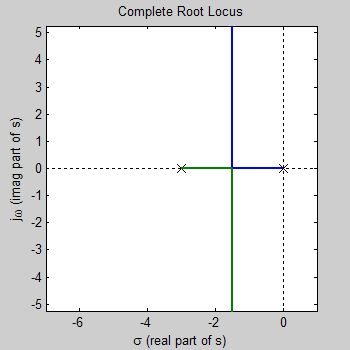
\includegraphics{./Root Locus_ Example 1_files/RLTotal.png}

\subsection[Root Locus
Symmetry]{\texorpdfstring{\protect\hypertarget{RuleSym}{}{}Root Locus
Symmetry}{Root Locus Symmetry}}\label{root-locus-symmetry}

As you can see, the locus is symmetric about the real axis\\

\subsection[Number of
Branches]{\texorpdfstring{\protect\hypertarget{RuleNum}{}{}Number of
Branches}{Number of Branches}}\label{number-of-branches}

The open loop transfer function, G(s)H(s), has 2 poles, therefore the
locus has 2 branches. Each branch is displayed in a different color.\\

\subsection[Start/End
Points]{\texorpdfstring{\protect\hypertarget{RuleStart}{}{}Start/End
Points}{Start/End Points}}\label{startend-points}

Root locus starts (K=0) at poles of open loop transfer function,
G(s)H(s).~ These are shown by an 'x' on the diagram
above\\[2\baselineskip]As $K\rightarrow \infty$ the location of closed loop poles move to
the zeros of the open loop transfer function, G(s)H(s). Don't forget we
have we also have q=n-m=2 zeros at infinity.~ (We have n=2 finite poles,
and m=0 finite zeros).\\

\subsection[Locus on Real
Axis]{\texorpdfstring{\protect\hypertarget{RuleReal}{}{}Locus on Real
Axis}{Locus on Real Axis}}\label{locus-on-real-axis}

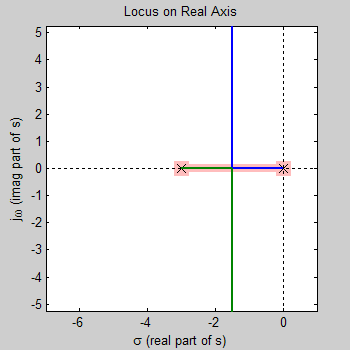
\includegraphics{./Root Locus_ Example 1_files/RLRealAxis.png}

The root locus exists on real axis to left of an odd number of poles and
zeros of open loop transfer function, G(s)H(s), that are on the real
axis.~~ These real pole and zero locations are highlighted on diagram,
along with the portion of the locus that exists on the real axis.

Root locus exists on real axis between:\\
0 and -3\\[2\baselineskip]\ldots{} because on the real axis, we have 2
poles at s = -3, 0, and we have no zeros.\\

\subsection[Asymptotes as \textbar{}s\textbar{} goes to
infinity]{\texorpdfstring{\protect\hypertarget{RuleInf}{}{}Asymptotes as
\textbar{}s\textbar{} goes to
infinity}{Asymptotes as \textbar{}s\textbar{} goes to infinity}}\label{asymptotes-as-s-goes-to-infinity}

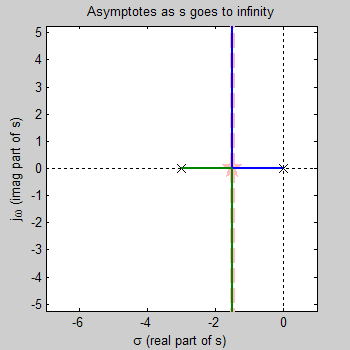
\includegraphics{./Root Locus_ Example 1_files/RLAsymptotes.png}

In the open loop transfer function, G(s)H(s), we have n=2 finite poles,
and m=0 finite zeros, therefore we have q=n-m=2 zeros at
infinity.\\[2\baselineskip]Angle of asymptotes at odd multiples of
±180°/q, (i.e., ±90°)\\[2\baselineskip]There exists 2 poles at s = 0,
-3, \ldots{}so sum of poles=-3.\\
There exists 0 zeros, \ldots{}so sum of zeros=0.\\
(Any imaginary components of poles and zeros cancel when summed because
they appear as complex conjugate pairs.)\\[2\baselineskip]Intersect of
asymptotes is at ((sum of poles)-(sum of zeros))/q = -1.5.\\
Intersect is at ((-3)-(0))/2 = -3/2 = -1.5 (highlighted by five pointed
star).\\

\subsection[Break-Out and In Points on Real
Axis]{\texorpdfstring{\protect\hypertarget{RuleBrk}{}{}Break-Out and In
Points on Real
Axis}{Break-Out and In Points on Real Axis}}\label{break-out-and-in-points-on-real-axis}

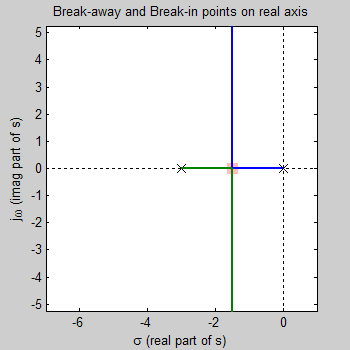
\includegraphics{./Root Locus_ Example 1_files/RLBreakOutIn.png}

Break Out (or Break In) points occur where N(s)D'(s)-N'(s)D(s)=0, or 2 s
+ 3 = 0. (details below*)\\[2\baselineskip]This polynomial has 1 root at
s = -1.5.\\[2\baselineskip]From these 1 root, there exists 1 real root
at s = -1.5.~ These are highlighted on the diagram above (with squares
or diamonds.)\\[2\baselineskip]These roots are all on the locus (i.e.,
K\textgreater{}0), and are highlighted with squares.\\[2\baselineskip]*
N(s) and D(s) are numerator and denominator polynomials of G(s)H(s), and
the tick mark, ', denotes differentiation.\\
N(s) = 1\\
N'(s) = 0\\
D(s)= s\textsuperscript{2} + 3 s\\
D'(s)= 2 s + 3\\
N(s)D'(s)= 2 s + 3\\
N'(s)D(s)= 0\\
N(s)D'(s)-N'(s)D(s)= 2 s + 3\\[2\baselineskip]Here we used
N(s)D'(s)-N'(s)D(s)=0, but we could multiply by -1 and use
N'(s)D(s)-N(s)D'(s)=0.\\

\subsection[Angle of
Departure]{\texorpdfstring{\protect\hypertarget{RuleDep}{}{}Angle of
Departure}{Angle of Departure}}\label{angle-of-departure}

No complex poles in loop gain, so no angles of departure.\\

\subsection[Angle of
Arrival]{\texorpdfstring{\protect\hypertarget{RuleArv}{}{}Angle of
Arrival}{Angle of Arrival}}\label{angle-of-arrival}

No complex zeros in loop gain, so no angles of arrival.\\

\subsection[Cross Imag.
Axis]{\texorpdfstring{\protect\hypertarget{RuleImag}{}{}Cross Imag.
Axis}{Cross Imag. Axis}}\label{cross-imag.-axis}

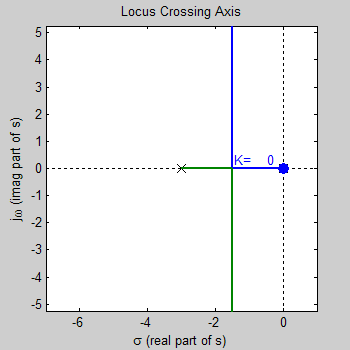
\includegraphics{./Root Locus_ Example 1_files/RLCrossImag.png}

Locus crosses imaginary axis at 1 value of K.~ These values are normally
determined by using Routh's method.~ This program does it numerically,
and so is only an estimate.\\[2\baselineskip]Locus crosses where K = 0,
corresponding to crossing imaginary axis at s=0.\\[2\baselineskip]These
crossings are shown on plot.\\

\subsection[Changing K Changes Closed Loop
Poles]{\texorpdfstring{\protect\hypertarget{RuleFindPole}{}{}Changing K
Changes Closed Loop
Poles}{Changing K Changes Closed Loop Poles}}\label{changing-k-changes-closed-loop-poles}

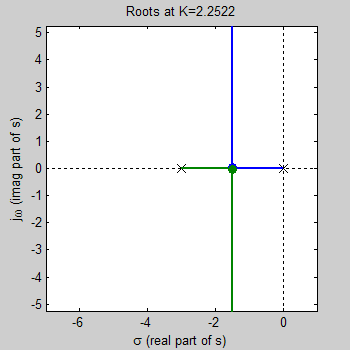
\includegraphics{./Root Locus_ Example 1_files/RLLocPos.png}

Characteristic Equation is 1+KG(s)H(s)=0, or 1+KN(s)/D(s)=0,\\
or D(s)+KN(s) = s\textsuperscript{2} + 3 s+ K( 1 ) =
0\\[2\baselineskip]So, by choosing K we determine the characteristic
equation whose roots are the closed loop poles.\\[2\baselineskip]For
example with K=2.25225, then the characteristic equation is\\
D(s)+KN(s) = s\textsuperscript{2} + 3 s + 2.2522( 1 ) = 0, or\\
s\textsuperscript{2} + 3 s + 2.2522= 0\\[2\baselineskip]This equation
has 2 roots at s = -1.5 ±0.047j.~ These are shown by the large dots on
the root locus plot\\

\subsection[Choose Pole Location and Find
K]{\texorpdfstring{\protect\hypertarget{RuleFindK}{}{}Choose Pole
Location and Find
K}{Choose Pole Location and Find K}}\label{choose-pole-location-and-find-k}

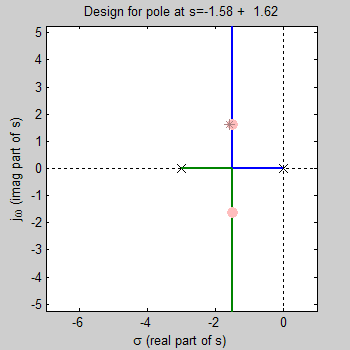
\includegraphics{./Root Locus_ Example 1_files/RLFindGain.png}

Characteristic Equation is 1+KG(s)H(s)=0, or 1+KN(s)/D(s)=0, or\\
K = -D(s)/N(s) = -( s\textsuperscript{2} + 3 s ) / ( 1 )\\
We can pick a value of s on the locus, and find
K=-D(s)/N(s).\\[2\baselineskip]For example if we choose s= -1.6 + 1.6j
(marked by asterisk),\\
then D(s)=-4.87 + -0.243j, N(s)= 1 + 0j,\\
and K=-D(s)/N(s)= 4.87 + 0.243j.\\
This s value is not exactly on the locus, so K is complex, (see note
below), pick real part of K ( 4.87)\\[2\baselineskip]For this K there
exist 2 closed loop poles at s = -1.5 ± 1.6j.~ These poles are
highlighted on the diagram with dots, the value of ``s'' that was
originally specified is shown by an asterisk.\\[2\baselineskip]Note: it
is often difficult to choose a value of s that is precisely on the
locus, but we can pick a point that is close.~ If the value is not
exactly on the locus, then the calculated value of K will be complex
instead of real. Just ignore the the imaginary part of K (which will be
small).~

Note also that only one pole location was chosen and this determines the
value of K. If the system has more than one closed loop pole, the
location of the other poles are determine solely by K, and may be in
undesirable locations.



\section[ \\
The Root Locus
Rules]{\texorpdfstring{\protect\hypertarget{SECTION00080000000000000000}{}{~}
		\protect\hypertarget{app.rlrules}{}{~}\\
		The Root Locus
		Rules}{~ ~ The Root Locus Rules}}\label{the-root-locus-rules}

To assist in the construction of root locus plots, the
``\protect\hypertarget{2261}{}{~}Root Locus Rules'' for plotting the
loci are summarized here. These rules are not universal, and every
author has his own favorite set and ordering of the rules. In his
landmark textbook, Walter Evans\protect\hypertarget{2250}{}{~} lists
approximately ten rules, but does not order or number them
{[}\href{http://www.mit.edu/people/klund/weblatex/node10.html\#evans54}{1},
Appendix B{]}, while Roberge\protect\hypertarget{2252}{}{~} enumerates
eight rules
{[}\href{http://www.mit.edu/people/klund/weblatex/node10.html\#roberge}{9},
pages 121-126{]}.

All root locus rules can be directly traced to the characteristic
equation, 1+\emph{L}(\emph{s})=0. If we assume that the loop transfer
function can be written as
\emph{L}(\emph{s})=\emph{KL}\textsubscript{0}(\emph{s}), where \emph{K}
is a positive gain, then we can write the magnitude condition and the
angle condition as\\

\textbar{}\emph{L}(\emph{s})\textbar{}=\textbar{}\emph{KL}\textsubscript{0}(\emph{s})\textbar{}=1

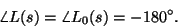
\includegraphics[width=1.85417in,height=0.29167in]{./The Root Locus Rules_files/img46.png}

We assume that the loop transfer function has \emph{P} open loop poles
and \emph{Z} open loop zeros, and that there are at least as many poles
as zeros
(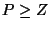
\includegraphics[width=0.51042in,height=0.30208in]{./The Root Locus Rules_files/img47.png}).

\begin{description}
	\item[\textbf{Rule 1} ]
	The number of branches, which are the paths of the closed-loop poles, is
	equal to the number of open-loop poles, \emph{P}.
	\item[\textbf{Rule 2} ]
	The branches start at the open-loop poles and end at the open-loop
	zeros. In addition to the \emph{Z} explicit open-loop zeros in the
	transfer function, there are \emph{P}-\emph{Z} open-loop zeros at
	infinity.
	\item[\textbf{Rule 3} ]
	Branches of the root locus lie on the real axis to the left of an odd
	number of poles and zeros. Complex-conjugate pairs of poles and zeros
	are not counted, since they contribute no net angle to the real axis.
	\item[\textbf{Rule 4} ]
	If a branch on the real axis lies between a pair of poles, the root
	locus must break away from the real axis somewhere between the poles.
	Similarly, if a branch on the real axis lies between a pair of zeros,
	there must be an entry point between that pair of zeros.
	\item[\textbf{Rule 5} ]
	As \emph{K} gets very large, \emph{P}-\emph{Z} branches go to infinity.
	These branches approach asymptotes at angles to the real axis of\\
	
	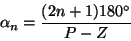
\includegraphics[width=1.36458in,height=0.42708in]{./The Root Locus Rules_files/img1.png}
	
	where
	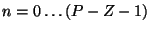
\includegraphics[width=1.56250in,height=0.32292in]{./The Root Locus Rules_files/img2.png}
	and the centroid of these asymptotes is on the real axis at\\
	
	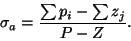
\includegraphics[width=1.36458in,height=0.42708in]{./The Root Locus Rules_files/img3.png}
	\item[\textbf{Rule 6} ]
	The departure angles \protect\hypertarget{2277}{}{~} of the branches
	from an \emph{m}th-order pole on the real axis are\\
	
	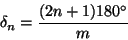
\includegraphics[width=1.33333in,height=0.41667in]{./The Root Locus Rules_files/img4.png}
	
	if the \emph{m}th-order pole is to the left of a even number of poles
	and zeros. If the \emph{m}th-order pole is to the left of a odd number
	of poles and zeros, then the departure angles are\\
	
	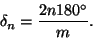
\includegraphics[width=0.96875in,height=0.40625in]{./The Root Locus Rules_files/img5.png}
	\item[\textbf{Rule 7} ]
	If there are two or more excess poles than zeros (
	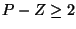
\includegraphics[width=0.79167in,height=0.30208in]{./The Root Locus Rules_files/img6.png}),
	then for any gain \emph{K}, the sum of the real parts of the closed-loop
	poles (or the average distance from the
	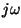
\includegraphics[width=0.21875in,height=0.29167in]{./The Root Locus Rules_files/img7.png}-axis)
	is
	constant\href{http://www.mit.edu/people/klund/weblatex/footnode.html\#foot2284}{\textsuperscript{3}}.
	\item[\textbf{Rule 8} ]
	Ignore remote poles and zeros when considering the root locus near the
	origin of the \emph{s}-plane, and combine the poles and zeros near the
	origin when considering the root locus for remote poles and zeros.
	\item[\textbf{Rule 9} ]
	The departure angle from a complex-conjugate pole can be found by
	considering the angle condition on a small circle around the pole. The
	result is found by summing all the angles from open-loop zeros and
	subtracting all the angles from all other poles\\
	
	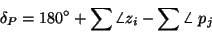
\includegraphics[width=2.20833in,height=0.34375in]{./The Root Locus Rules_files/img8.png}
	
	The approach angle to a complex-conjugate zero follows similarly\\
	
	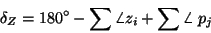
\includegraphics[width=2.19792in,height=0.34375in]{./The Root Locus Rules_files/img9.png}
	
	This sum only needs to be calculated once for each complex pair, since
	the root-locus diagram is symmetric above and below the real axis.
	\item[\textbf{Rule 10} ]
	The break-away (entry) points from (to) the real axis between a pair of
	poles (zeros) can be found either by geometric
	construction\href{http://www.mit.edu/people/klund/weblatex/footnode.html\#foot2293}{\textsuperscript{4}}
	or by finding the local maxima (minima) of the gain function
	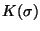
\includegraphics[width=0.41667in,height=0.32292in]{./The Root Locus Rules_files/img10.png},
	solving \protect\hypertarget{2294}{}{~}\\
	
	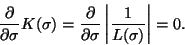
\includegraphics[width=1.92708in,height=0.46875in]{./The Root Locus Rules_files/img11.png}
	
	Fortunately, this level of accuracy is rarely necessary.
\end{description}

\end{document}
